\ofsubsection{Jobs}
%
%
%
%
%
\ofjob{Bard}
{
	\ofquote{"Welcome to your doom, starring me!"\\}{Rikku}\\\\
	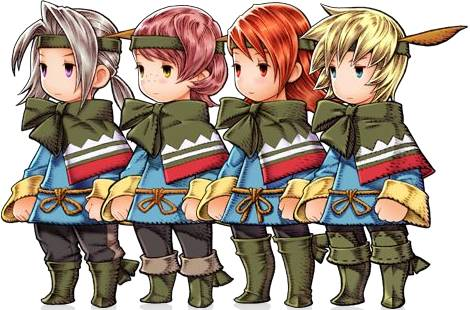
\includegraphics[width=\columnwidth]{./art/jobs/bard.jpg}\ofrow
	\accf{Bards} blur the lines between art and war.
	They can perform songs and dances that bestow powerful benefits for allies and vicious handicaps for enemies.
	Even though Bards are not the most powerful duelists, they can often turn the tide of a battle in unexpected ways.
}
{Dagger}{Light Armor or Robe}{
	Level 1: & HP~+19 & MP~+20 & AGI~+3 & RES~+1  \\
	Level 2: & HP~+10  & MP~+10 & DEF~+1  \\
	Level 3: & \multicolumn{3}{l}{Archetype Attribute Bonus} \\
	Level 4: & HP~+5  & MP~+10 & RES~+1 & DEF~+1 \\
	Level 5: & HP~+10 & MP~+5  & STR~+2 \\ 
	Level 6: & HP~+5  & MP~+10 & RES~+1 & DEF~+1 \\
	Level 7: & HP~+10 & MP~+10 & STR~+1 &  	  \\
	Level 8: & HP~+10  & MP~+10 & DEF~+1 \\
	Level 9: & HP~+10 & MP~+10 & STR~+1 \\
	Level 10: & HP~+5  & MP~+10 & RES~+1 & DEF~+1	
}{
	\ofjobtech{Cheer}{4}{0r}{1u}{Self}{Everyone in the target area can choose to either gain \mbox{EnSTR}, EnMAG, EnDEF or EnRES for 3 rounds.}{\enstr\enmag}{1}\ofabilitygap
	\ofjobtech{Improvise}{6}{0r}{Single}{5u}{Roll 1d. Based on the result, the target gains the following Status Effect for 3 rounds:\\ 1-EnDEF, 2-EnRES, 3-EnSTR, 4-Blink, 5-Regen, 6-Haste.}{\enndef\enres\enstr\blink\regen\haste}{2}\ofabilitygap
	\ofjobtech{Spotlight}{8}{0r}{2u}{Self}{You create an Obscure Field around yourself that follows you for 3 rounds, but does not affect you.}{}{4}\ofabilitygap
	\ofjobtech{Mighty March}{12}{0r}{2u}{Self}{You and all allies in the target area gain Haste and EnDEF for 2 rounds.}{\haste\enndef}{6}\ofabilitygap
	\ofjobtech{Charm}{14}{1r}{Single}{4u}{Choose an enemy as the target. He makes a DC~8 check and upon failure he immediately takes an extra turn following your command. The turn order is unchanged. Some enemies may be Immune to this effect.}{}{8}\ofabilitygap
	\ofjobtech{Mimic}{?}{0r}{?}{?}{You use an ability that was used by an ally or enemy on the battlefield since your last turn. In doing this, you have to respect the MP cost, cast time as well as the target and range specifications of the copied ability.}{}{10}
}{
	\ofarchetypet{Dancer}
	{HP~+12 & MP~+8 & STR~+2 & DEF~+1}
	{\ofarchetypetecha{Blade Dance}{6}{0r}{Single}{1u}{Make an Attack on the target. Then you can immediately choose another target within 2u, dash towards him and make an Attack on him as well.}{}}
	{\ofspecial{Dress to Impress}{You can equip one additional Accessory. Also, for each equipped Accessory you can choose to gain either an additional DEF +1 or RES +1.}{5}{\oficonpassive}}	
	{\ofspecial{Dirty Dancing}{Whenever you successfully evade an Attack, you can immediately inflict one of the following Status Effects on the attacker for 3 rounds: Immobile, Poison, Blind.}{7}{\oficonreaction}}
	{\ofarchetypetechb{Slow Dance}{12}{0r}{2u}{Self}{You create a special Field around yourself that lasts for 3 rounds and simultaneously acts as a Slow Field and Hot Field. The Field moves together with you and it only affects enemies.}{}}
}{
	\ofarchetypet{Singer}
	{HP~+4 & MP~+16 & RES~+3}
	{\ofarchetypetecha{Requiem}{8}{0r}{Single}{4u}{The target makes a DC~8 check and upon failure he suffers dark damage equal to two times your current Level and Zombie for 3 rounds.}{\zombie\dark}}
	{\ofarchetypepassive{Encore}{Whenever you bestow one or more positive Status Effects on a target, additionally restore his HP by an amount equal to your current Level.}}
	{\ofarchetypereaction{Duet}{Whenever an ally within 1u of you performs an Attack or uses an ability on an enemy, you can immediately use any ability either on your ally or on the affected target if he is within range.}}
	{\ofarchetypetechb{Lullaby}{12}{0r}{2u}{5u}{All enemies in the target area make a DC~8 check and suffer 3d damage and Sleep for 3 rounds upon failure.}{\sleep}}
}
%
%
%
%
%
\ofjob{Black Mage}
{
	\ofquote{"You sure are a keen observer of the obvious, kupo!"\\}{Montblanc}\\\\
	
\includegraphics[width=\columnwidth]{./art/jobs/blackmage2.jpg}\ofrow
	\accf{Black Mages} are fragile in physical combat, but can wipe out enemies from great distances with powerful magic. 
	They assert great control over the battlefield and are difficult to ignore for enemies. 
}
{Rod}{Robe}{
	Level 1: & HP~+18 & MP~+26 & AGI~+2 & RES~+1  \\
	Level 2: & HP~+5  & MP~+10 & MAG~+1 & STR~+1  \\
	Level 3: & \multicolumn{3}{l}{Archetype Attribute Bonus} \\
	Level 4: & MP~+10 & RES~+1 & DEF~+1 & MAG~+1 	\\
	Level 5: & HP~+10 & MP~+10 & MAG~+1 		  \\
	Level 6: & HP~+5  & MP~+10 & RES~+1 & MAG~+1 \\
	Level 7: & HP~+5  & MP~+10 & MAG~+1 & RES~+1 \\
	Level 8: & HP~+5  & MP~+10 & RES~+1 & DEF~+1 \\
	Level 9: & HP~+5  & MP~+10 & RES~+1 & MAG~+1  \\
	Level 10: & HP~+10 & MP~+10 & MAG~+1		  
}{
	\ofjobspell{Fire}{4}{0r}{Single}{3u}{You deal 2d fire damage to the target.}{\fire}{1}\ofabilitygap
	\ofjobspell{Blizzard}{4}{0r}{Single}{3u}{You deal 2d ice damage to the target.}{\ice}{1}\ofabilitygap
	\ofjobspell{Thunder}{4}{0r}{Single}{3u}{You deal 2d lightning damage to the target.}{\lightning}{1}\ofabilitygap
	\ofjobspell{Blind}{6}{0r}{Single}{5u}{The target makes a DC 8 check and suffers Blind for 3 rounds upon failure.}{\blind}{2}\ofabilitygap
	\ofjobspell{Firaga}{12}{1r}{Single}{5u}{You deal 6d fire damage to the target.}{\fire}{6}\ofabilitygap
	\ofjobspell{Blizzaga}{12}{1r}{Single}{5u}{You deal 6d ice damage to the target.}{\ice}{6}\ofabilitygap
	\ofjobspell{Thundaga}{12}{1r}{Single}{5u}{You deal 6d lightning damage to the target.}{\lightning}{6}\ofabilitygap
	\ofjobspell{Flare}{20}{2r}{Single}{10u}{You deal 6d+50 damage to the target. The damage dealt ignores the target's RES.}{\fire}{8}\ofabilitygap
	\ofjobspell{Ultima}{30}{2r}{50u}{Self}{Deal 6d+40 dark damage to all enemies in the target area.}{\dark}{10}
}{
	\ofarchetypet{Geomancer}
	{HP~+14 & MP~+6 & DEF~+2 & RES~+1}
	{\ofarchetypespella{Bio}{8}{0r}{Single}{5u}{The target makes a DC 8 check and suffers 3d damage and Poison for 3 rounds upon failure.}{\poison}}
	{\ofarchetypepassive{Field Cast}{Whenever you cast a spell that deals fire, ice or lightning elemental damage, it also creates a Field around the target that reaches up to 2u and lasts for 1 round. The Field effect depends on the elemental type of the spell:\\ Fire - Hot Field, Ice - Slippery Field, Lightning - Slow Field.}}
	{\ofarchetypereaction{Gaia's Shield}{Whenever you suffer elemental damage, double your DEF and RES for calculating the damage received.}}
	{\ofarchetypespellb{Quake}{18}{1r}{3u}{10u}{Deal 6d+5 earth damage to everyone in the target area.}{\earth}}
}{
	\ofarchetypet{Scholar}
	{HP~+7 & MP~+18 & MAG~+2}
	{\ofarchetypespella{Zombify}{8}{0r}{Single}{5u}{The target makes a DC 8 check and suffers 3d dark damage and Zombie for 3 rounds upon failure.}{\zombie}}
	{\ofarchetypepassive{Study}{Whenever you deal magical damage to an enemy, you can choose one of the following aspects that you learn about him: Resiliences, Weaknesses, Immunities, current HP, current MP.}}
	{\ofarchetypereaction{Learn}{Whenever you are targeted by Magic, you can make a DC~8 check. If you succeed, you learn how to use the same spell. If you have already learned a spell in this way, you can choose to forget it to learn a new one.}}
	{\ofarchetypespellb{Doom}{18}{0r}{Single}{8u}{The target makes a DC 8 check and suffers KO after 3 rounds upon failure. If the enemy is Immune to KO, he instead suffers 6d+5 dark damage.}{\ko}}
}
%
%
%
%
%
\ofjob{Dragoon}
{
	\ofquote{"Confident bastard, aren't you?"\\}{Kain}\\\\
	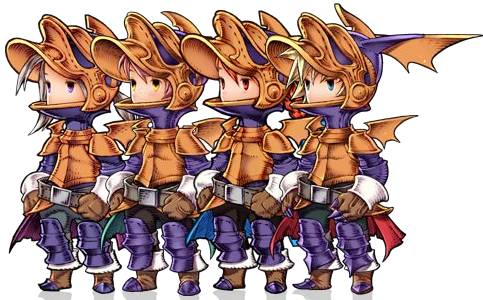
\includegraphics[width=\columnwidth]{./art/jobs/dragoon.jpg}\ofrow
	\accf{Dragoons} are masters of aerial combat, who strike their enemies with devastating attacks from the sky.
	They prefer spears as their weapon and have an affinity for the fire element. 
	Even though they are humanoid, it is said that Dragoons have the soul of a dragon.
}
{Spear}{Heavy Armor}{
	Level 1: & HP +23 & MP~+16 & AGI~+2,& STR~+1 \\
	Level 2: & HP~+10  & MP~+5 & STR~+1 & RES~+1 \\
	Level 3: & \multicolumn{3}{l}{Archetype Attribute Bonus} \\
	Level 4: & HP~+5  & MP~+10 & DEF~+2 &  	  \\
	Level 5: & HP~+10 & MP~+10 & STR~+1 & 		  \\ 
	Level 6: & HP~+10 & MP~+10 & RES~+1 		  \\
	Level 7: & HP~+10 & MP~+5  & STR~+1 & 	DEF~+1	  \\ 
	Level 8: & HP~+10 & MP~+10 & RES~+1 & 	 	  \\ 
	Level 9: & HP~+10  & MP~+10 & STR~+1 \\ 
	Level 10:& HP~+10  & RES~+1 & DEF~+2 
}{
	\ofjobtech{Jump}{4}{1r}{Single}{3u}{When you begin using this Tech, you jump 3u up into the air. After the cast time is up, you leap onto the target and make an Attack on him.}{}{1}\ofabilitygap
	\ofjobtech{Lancet}{3}{0r}{Single}{5u}{You deal damage to the target's HP and MP by an amount equal to your current Level and increase your own HP and MP by the same amount. This amount is not recued by the target's DEF or RES.}{}{2}\ofabilitygap
	\ofjobtech{Double Jump}{8}{1r}{Single}{3u}{When you begin using this tech, you jump 3u up into the air. After the cast time is up, you leap onto the target and make an Attack on him. You can then leap to another location within 3u. If you land on another enemy you can make an Attack on him too.}{}{6}\ofabilitygap
	\ofjobtech{Roar}{8}{0r}{5u}{Self}{All enemies in the target area make a DC 9 check and suffer 2d damage and Immobile for 1 round upon failure.}{\immobile}{8}\ofabilitygap
	\ofjobtech{Highwind}{24}{1r}{Single}{Self}{For the next 3 rounds, you stay up to 3u in the air from where you can move your usual distance and perform one of the following 2 actions without additional MP cost or cast time on each turn:\\ 
		\acc{Lance Barrage:} make an Attack against a target within 10u. If you hit, you score a Critical Hit.\\
		\acc{Fire Blast:} choose a target within 10u. He and all enemies within 2u of him suffer 4d fire damage.
	}{\fire}{10}
}{
	\ofarchetypet{Dragon Knight}
	{HP~+8 & MP~+12 & STR~+1 & RES~+2}
	{\ofarchetypetecha{Fire Breath}{7}{0r}{3u (front)}{Self}{You deal 2d fire damage to everyone in the target area.}{\fire}}
	{\ofarchetypepassive{Flametongue}{You gain permanent Resilience against fire damage. Furthermore, whenever you deal physical damage to an enemy, you can choose to let the damage dealt be of magical and fire type instead.}}
	{\ofarchetypereaction{Dragonheart}{Whenever you deal or receive fire damage, you gain EnSTR until the end of your next turn.}}
	{\ofarchetypetechb{Dragon Dive}{16}{1r}{3u}{7u}{When you begin using this Tech, you jump 3u up into the air. After the cast time is up you leap onto the target and deal 4d fire damage to everyone in the target area except yourself. Also, you create Hot Field in the target area that lasts for 3 rounds but does not affect you.}{\fire}}
}{
	\ofarchetypet{Valkyrie}
	{HP~+13 & MP~+7 & STR~+2 & DEF~+1}
	{\ofarchetypetecha{Full Thrust}{6}{0r}{5u (line)}{Self}{You dash forward in an up to 5u long line. Make an Attack on everyone in the way by making one damage roll that is applied to all targets that fail to evade.}{}}
	{\ofarchetypepassive{Duelist}{As long as you are in combat within 3u of one enemy and there is noone else within 3u of you, the STR bonus added to your Attacks and Abilities is doubled.}}
	{\ofarchetypereaction{Arm's Length}{Whenever an enemy walks within 2u of you, he has to make a DC~7 check and upon failure he cannot move any further towards you on this turn.}}
	{\ofarchetypetechb{Revenge}{16}{0r}{Single}{1u}{Make an Attack on an enemy that has damaged you since your last turn. On hit, you inflict the damage that he dealt to you before instead of your usual damage.}{}}
}
%
%
%
%
%
\ofjob{Marksman}
{
	\ofquote{"I play the leading man; who else?"\\}{Balthier}\\\\
	
\includegraphics[width=\columnwidth]{./art/jobs/marksman.jpg}\ofrow
	\accf{Marksmen} are experts of all kinds of ranged weapons that strike from great distance. 
	Skilled Marksmen can see through their enemies, allowing them to know a target's strengths and weaknesses. 
	Therefore they can not only deal significant ranged damage, but also disable enemies with special techniques.
}
{Bow or Gun}{Light Armor}{
	Level 1: & HP +19 & MP~+17 & AGI~+2 & STR +1 \\
	Level 2: & HP~+10  & MP~+10 & DEF~+1 \\
	Level 3: & \multicolumn{3}{l}{Archetype Attribute Bonus}  \\
	Level 4: & HP~+5  & MP~+5  & STR~+2 & RES~+1 \\
	Level 5: & HP~+5  & MP~+10 & DEF~+1 & RES~+1  \\
	Level 6: & HP~+10 & MP~+10 & RES~+1 &        \\
	Level 7: & HP~+5  & MP~+10 & STR~+1 & RES~+1 \\
	Level 8: & HP~+10  & MP~+5 & DEF~+2 		  \\
	Level 9: & HP~+5  & MP~+10 & RES~+1 & STR~+1 \\
	Level 10:& HP~+10 & MP~+10 & STR~+1 &        
}{
	\ofjobtech{Libra}{4}{0r}{Single}{5u}{You analyse the target thoroughly and know his Resiliences, Weaknesses, Immunities, as well as his current HP and MP.}{}{1}\ofabilitygap
	\ofjobtech{Heavy Shot}{6}{0r}{Single}{Weapon}{Make an Attack on the target. If you hit, the damage dealt ignores the target's DEF.}{}{2}\ofabilitygap
	\ofjobtech{Fast Draw}{8}{0r}{Single}{Weapon}{You make an Attack after which you can immediately begin using another Ability in the same turn.}{}{4}\ofabilitygap
	\ofjobtech{Explosive Shot}{10}{0r}{2u}{Weapon}{Everyone in the target area suffers 3d fire damage. In addition, you create a Hot Field in the target area that lasts for 3 rounds.}{\fire}{6}\ofabilitygap
	\ofjobtech{Smoke Bomb}{10}{0r}{3u}{10u}{You create an Obscure Field in the target area that lasts for 3 rounds.}{}{8}\ofabilitygap
	\ofjobtech{Barrage}{22}{1r}{Single}{Self}{You gain Haste and EnSTR for 3 rounds. Also, all your Attacks which target a single enemy instead affect all enemies within 2u of the chosen target.
	}{\haste\enstr}{10}
}{
	\ofarchetypet{Ranger}
	{HP~+13 & MP~+12 & DEF~+2}
	{\ofarchetypetecha{Lay Trap}{5}{0r}{1u}{Self}{You set a trap where you are standing. An enemy that walks over it suffers damage equal to your current Level and Immobile for 1 round. The trap disappears once it is activated.}{\immobile}}
	{\ofarchetypepassive{Recoil}{Whenever you make a successful Attack, you can immediately move 1u in any direction.}}
	{\ofarchetypereaction{Magic Evade}{You can evade Magic by passing an evasion check. When you evade an Attack or Magic, you also regain an amount of MP equal to your current Level.}}
	{\ofarchetypetechb{Poison Ammo}{10}{0r}{Single}{Weapon}{Make an Attack on the target. If you hit, the damage dealt is magical and the target makes a DC 8 check. Upon failure, he suffers Poison, DeSTR and DeDEF for 3 rounds.}{\poison\destr\dedef}}
}{
	\ofarchetypet{Sniper}
	{HP~+5 & MP~+15 & STR~+3}
	{\ofarchetypetecha{Pierceshot}{6}{0r}{10u (line)}{Self}{Make an Attack against all targets in a line, by making one damage roll that applies to everyone that fails to evade.}{}}
	{\ofarchetypepassive{Concentrate}{Whenever you Attack an enemy, he has Disadvantage on the evasion check.}}
	{\ofarchetypereaction{Camouflage}{Whenever you end a turn in which you have not moved, you gain Blink until the start of your next turn.}}
	{\ofarchetypetechb{Aim}{8}{0r}{Single}{Weapon}{Make an Attack on the target and choose one of the following spots to inflict an additional effect if you hit:\\ \acc{Head:} the target's evasion DC is reduced by 2, but if you hit you score a Critical Hit.\\ \acc{Heart:} the target's MP is reduced by same amount as HP.\\ \acc{Leg:} the target suffers Immobile for 1 round.}{\immobile}}
}
%
%
%
%
%
\ofjob{Monk}
{
	\ofquote{"Now I know why I have these stupid muscles!"\\}{Sabin}\\\\
	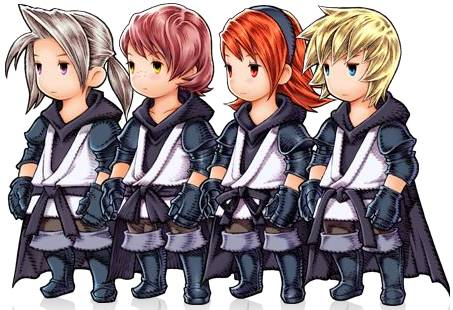
\includegraphics[width=\columnwidth]{./art/jobs/monk2.jpg}\ofrow
	\accf{Monks} are adept melee fighters that posses a deadly combination of strength and technique.
	While they do not have expertise in using magic, Monks can produce similar effects by tapping into their inner life force. 
}
{None}{Light Armor}{
	Level 1: & HP +20 & MP~+13 & AGI~+4 & \\
	Level 2: & HP~+10 & MP~+5  & STR~+2 & \\
	Level 3: & \multicolumn{3}{l}{Archetype Attribute Bonus} \\
	Level 4: & HP~+5  & MP~+10 & STR~+1 & RES~+1 \\
	Level 5: & HP~+10  & MP~+5 & DEF~+1 & STR~+1 \\
	Level 6: & HP~+10 & MP~+5  & STR~+1 & RES~+1 \\
	Level 7: & HP~+10 & MP~+5  & STR~+1 & DEF~+1 \\ 
	Level 8: & HP~+10 & MP~+5  & DEF~+2 &        \\
	Level 9: & HP~+5  & MP~+10 & STR~+1 & RES~+1 \\ 
	Level 10: & HP~+10 & MP~+10 & DEF~+1 &        \\ 
}{
	\ofjobpassive{Brawler}{In combat, you can use your bare fists as your weapon. They have the same DMG as weapons of the highest equipment rank that you can use. In addition, you can carry a third Accessory in place of your weapon slot and you gain STR +1 for every equipped Accessory. You may also slot materia onto the Accessory that you are carrying in place of a weapon.}{1}\ofabilitygap
	\ofjobtech{Kick}{4}{0r}{1u}{Self}{You make an Attack against all enemies within 1u of you, by making one damage roll that applies to all affected targets that fail to evade. All targets that fail to evade are also knocked back by 1u.}{}{2}\ofabilitygap
	\ofjobtech{Aurablast}{6}{0r}{Single}{3u}{You deal an amount of magical damage equal to your current Level to the target.}{}{4}\ofabilitygap
	\ofjobtech{Pummel}{8}{0r}{Single}{1u}{You make 2 consecutive Attacks against the target.}{}{6}\ofabilitygap
	\ofjobtech{Blitz}{3}{0r}{Single}{Self}{You use two different Techs consecutively in the same turn. In doing this, you have to respect additional MP costs and cast times of both Techs.}{}{8}\ofabilitygap
	\ofjobtech{Final Heaven}{22}{0r}{Single}{1u}{You deal 6d damage to the target and knock him back by 5u. If he hits a wall or a similarly solid object in doing so, you deal another 3d damage to him.}{}{10}
}{
	\ofarchetypet{Black Belt}
	{HP~+17 & MP~+8 & STR~+2}
	{\ofarchetypetecha{Bonecrusher}{6}{0r}{Single}{1u}{Make an Attack against the target. On hit, the target makes a DC~8 check and suffers Slow for 1 round upon failure.}{\slow}}
	{\ofarchetypepassive{Unscarred}{As long as your current HP is equal to your maximum HP, the STR bonus that is added to the damage dealt by your Attacks is doubled.}}
	{\ofarchetypereaction{Strikeback}{When you successfully evade an Attack by an enemy, you immediately make an Attack on him, if he is within range.}}
	{\ofarchetypetechb{Meteor Strike}{14}{0r}{Single}{1u}{You slam the target into the ground dealing 5d damage. In doing this, you can also leap to a location of your choice within 3u.}{}}
}{
	\ofarchetypet{Templar}
	{HP~+4 & MP~+16 & DEF~+1 & RES~+2}
	{\ofarchetypetecha{Chakra}{6}{1r}{Single}{Self}{You regain an amount of HP equal to your current Level and recover from one Status Effect that you are currently suffering.}{}}
	{\ofarchetypepassive{Lifestream}{If you do not have enough MP to use an ability you can instead choose to reduce your HP by the amount of its MP cost in order to use it.}}
	{\ofarchetypereaction{Replenish MP}{Whenever you suffer physical damage, you regain an amount of MP equal to half your current Level.}}
	{\ofarchetypetechb{Revive}{14}{1r}{Single}{1u}{You remove KO from the target and increase his HP by~1.}{\ko}}
}
%
%
%
%
%
\ofjob{Red Mage}
{
	\ofquote{"Oh, I’ll show you how lightning strikes."\\}{Lightning}\\\\
	
\includegraphics[width=\columnwidth]{./art/jobs/redmage.jpg}\ofrow
	\accf{Red Mages} are very versatile and possess a wide variety of abilities, but can also hold their own in melee combat. 
}
{Rod or Sword}{Light Armor or Robe}{
	Level 1: & HP~+20 & MP~+21 & AGI~+3 & STR +1 \\
	Level 2: & HP~+5  & MP~+10 & MAG~+1 & DEF~+1 \\
	Level 3: & \multicolumn{3}{l}{Archetype Attribute Bonus}   \\
	Level 4: & HP~+10 & MP~+5  & STR~+1 & RES~+1 \\   
	Level 5: & HP~+5  & MP~+10 & MAG~+2 & 		  \\ 
	Level 6: & HP~+5 & MP~+10  & STR~+1 &	MAG~+1 \\ 
	Level 7: & HP~+10  & MP~+10 & DEF~+1 \\ 
	Level 8: & HP~+10 & MP~+5  & STR~+1 & MAG~+1 \\ 
	Level 9: & HP~+5  & MP~+10 & RES~+2 \\ 
	Level 10: & HP~+10 & MP~+10 & STR~+1 		  
}{	
	\ofjobspell{Fire}{4}{0r}{Single}{3u}{You deal 2d fire damage to the target.}{\fire}{1}\ofabilitygap
	\ofjobspell{Blizzard}{4}{0r}{Single}{3u}{You deal 2d ice damage to the target.}{\ice}{1}\ofabilitygap
	\ofjobspell{Thunder}{4}{0r}{Single}{3u}{You deal 2d lightning damage to the target.}{\lightning}{1}\ofabilitygap
	\ofjobspell{Regen}{6}{0r}{Single}{5u}{The target gains Regen for 3 rounds.}{}{2}\ofabilitygap
	\ofjobspell{Blind}{6}{0r}{Single}{5u}{The target makes a DC~8 check and suffers Blind for 3 rounds upon failure.}{\blind}{4}\ofabilitygap	
	\ofjobspell{Vox}{6}{0r}{Single}{5u}{Remove one Status Effects except KO from the target. Also, the target becomes Immune to that Status Effect for 5 rounds.}{}{6}\ofabilitygap
	\ofjobspell{Imperil}{8}{0r}{Single}{5u}{The target suffers DeDEF and DeRES for 3 rounds.}{}{8}\ofabilitygap
	\ofjobspell{Wall}{8}{0r}{Single}{5u}{The target gains EnDEF and EnRES for 3 rounds.}{}{8}\ofabilitygap
	\ofjobspell{Dualcast}{2}{0r}{Single}{Self}{You begin casting two spells of your choice simultaneously, but need to spend the necessary MP for both.}{}{10}
}{
	\ofarchetypet{Ravager}
	{HP~+6 & MP~+14 & MAG~+2 & RES~+1}
	{\ofarchetypespella{Osmosis}{0}{0r}{Single}{5u}{You regain MP equal to your MAG and the target's MP is reduced by the same amount.}{}}
	{\ofarchetypepassive{Overwhelm}{When you inflict elemental damage, the target gains a weakness against that type until the end of your next turn. If he has a Resilience against it, that is negated instead.}}
	{\ofarchetypereaction{Swiftcast}{Once per round, right after an enemy within 5u uses an action, you can immediately cast a spell on him.}}
	{\ofarchetypespellb{NulElement}{10}{0r}{Single}{5u}{Choose an element (e.g. fire). The target does not suffer any damage of the chosen element for 3 rounds.}{}}
}{
	\ofarchetypet{Spellblade}
	{HP~+14 & MP~+6 & STR~+2 & DEF~+1}
	{\ofarchetypetecha{Elemental Strike}{6}{0r}{Single}{1u}{Choose an element (e.g. fire) and make an Attack. If you hit, the damage is of magical type with the chosen element and you also add your MAG to the damage dealt.}{}}
	{\ofarchetypepassive{Magic Weapon}{Whenever you cast Magic, you can choose to store the spell inside your weapon. In this case, the spell's MP cost is halved. All stored spells take effect together with your next successful Attack and you can chose targets within their range including yourself. You cannot store more than two spells at once inside your weapon.}}
	{\ofarchetypereaction{Mana Shield}{Whenever your HP is reduced, you can instead choose to reduce your MP by the same amount.}}
	{\ofarchetypetechb{Magic Barrier}{10}{0r}{Single}{5u}{For the next 3 rounds, the target can evade the effect of spells and techs by passing an evasion check.}{}}
}
%
%
%
%
%
\ofjob{Sentinel}
{
	\ofquote{"Allow me to shatter your delusions of grandeur."\\}{Beatrix}\\\\
	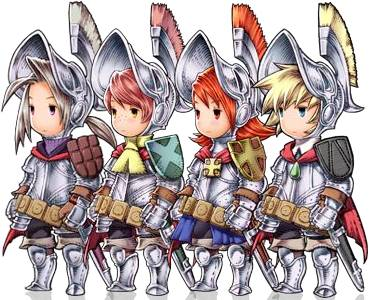
\includegraphics[width=\columnwidth]{./art/jobs/sentinel.jpg}\ofrow
	\accf{Sentinels} are masters of defensive combat who will rarely fall in a battle.  
	Their special abilities allow them to not only withstand incredible amounts of damage, but also provide protection to their allies.
	A capable Sentinel is often the last thing standing between the party and certain death.
}
{Sword}{Heavy Armor}{
	Level 1: & HP~+27 & MP~+18 & AGI~+3 & DEF~+1  \\
	Level 2: & HP~+10 & MP~+10 & STR~+1 & RES~+1 \\
	Level 3: & \multicolumn{3}{l}{Archetype Attribute Bonus} \\
	Level 4: & HP~+10 & MP~+5  &  DEF~+1 & STR~+1 \\ 
	Level 5: & HP~+10 & MP~+5  & RES~+1 & DEF~+1 \\ 
	Level 6: & HP~+10 & MP~+10 & STR +1 &        \\
	Level 7: & HP~+10 & MP~+5  & DEF +2 &        \\
	Level 8: & HP~+10 & MP~+5  & STR +1 & DEF~+1 \\
	Level 9: & HP~+10 & MP~+10 & STR +1 &        \\
	Level 10: & HP~+10  & MP~+10 & DEF +1 
}{
	\ofjobtech{Guard}{3}{0r}{Single}{Self}{You gain EnDEF until the end of your next turn.}{\enndef}{1}\ofabilitygap
	\ofjobtech{First Aid}{6}{1r}{Single}{1u}{%
		When you begin using this ability, the target regains an amount of HP equal to your current Level. After the cast time is up, if you have received no damage since casting and if the target is still in range, he additionally gains EnDEF and Haste for 1 round.}{}{2}\ofabilitygap
	\ofjobtech{Threaten}{8}{0r}{Single}{5u}{The target makes a DC 8 check and suffers Immobile for 3 rounds upon failure.}{\immobile}{4}\ofabilitygap
	\ofjobtech{Mediguard}{9}{0r}{Single}{Self}{You gain EnDEF and Regen for 3 rounds.}{\enndef}{6}\ofabilitygap
	\ofjobtech{Defensive Formation}{10}{0r}{2u}{Self}{You and all allies within the target area gain Blink for 2 rounds.}{\blink}{8}\ofabilitygap
	\ofjobtech{Mighty Guard}{26}{1r}{Single}{Self}{For the next 3 rounds, you gain Resilience against all physical and magical damage.}{}{10}
}{
	\ofarchetypet{Defender}
	{HP~+17 & MP~+3 & STR~+2 & DEF~+1}
	{\ofarchetypetecha{Powerbreak}{6}{0r}{Single}{1u}{Make an Attack on the target. If you hit, he suffers DeSTR and DeMAG for 2 rounds on top of the damage dealt.}{\destr \demag}}
	{\ofarchetypepassive{Provoke}{Whenever you successfully Attack an enemy, you can try to provoke him. If you do so, he has to make a DC~8 check and upon failure he has to target you with an action on his next turn if possible.}}
	{\ofarchetypereaction{Block}{Whenever an enemy within 2u of you tries to move away from you, he has make a DC 8 check. Upon failure, he suffers Immobile until the start of his next turn, preventing him from moving any further on this turn.}}
	{\ofarchetypetechb{Vengeance}{14}{0r}{Single}{1u}{The target suffers damage equal to half the difference between your current and your maximum HP.}{}}
}{
	\ofarchetypet{Paladin}
	{HP~+10 & MP~+15 & RES~+2}
	{\ofarchetypetecha{Earth Wall}{8}{0r}{3u (line)}{8u}{You create a 3u tall and wide wall of earth that blocks the path. The wall breaks down after 3 rounds or upon suffering a total of 20 damage. You cannot use this ability if a previous wall still exists.}{}}
	{\ofarchetypepassive{Holy Guard}{As long as there is at least one ally within 1u of you, you and all allies within 1u gain EnRES.}}
	{\ofarchetypereaction{Cover}{Whenever an ally within 1u of you receives physical damage, you can decide to direct half of the total damage dealt on yourself instead of onto your ally.}}
	{\ofarchetypetechb{Astra}{10}{0r}{Single}{5u}{For the next 3 rounds, the target gains EnRES and becomes Immune to all Status Effects.}{\enres}}
}
%
%
%
%
%
\ofjob{Summoner}
{
	\ofquote{"I don’t like your plan. It sucks."\\}{Yuna}\ofrow
	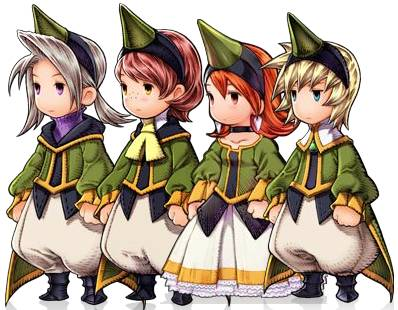
\includegraphics[width=\columnwidth]{./art/jobs/summoner.jpg}\ofrow
	Most powerful heroes are able to call creatures, but the bonds created \accf{Summoners} are far stronger allowing them
	manifest summons for a longer time to fight alongside them on the battlefield.
}
{Rod or Staff}{Robe}{
	Level 1: & HP +16 & MP~+24 & AGI~+2 & STR~+1 \\ 
	Level 2: & HP~+5  & MP~+10 & RES~+1 & MAG~+1 \\ 
	Level 3: & \multicolumn{3}{l}{Archetype Attribute Bonus}   \\
	Level 4: & HP~+5  & MP~+10 & RES~+1 & DEF~+1 \\ 
	Level 5: & HP~+5 & MP~+5  & RES~+2 & MAG~+1 \\  
	Level 6: & HP~+10 & MP~+10 & DEF~+1 \\  
	Level 7: & HP~+5 & MP~+10 & RES~+1 &  MAG~+1      \\  
	Level 8: & HP~+5 & MP~+10 & DEF~+1 &		  \\  
	Level 9: & HP~+10 & MP~+5  & MAG~+1 & RES~+1 \\  
	Level 10: & HP~+10 & MP~+10 & STR~+1 &        	  
}{
	\ofjobspell{Summon}{8}{1r}{1u}{1u}{
		You manifest a creature, that you have the ability to summon, on the battlefield.  
		In combat, summons take their turn right after yours, following your command.
		They are dismissed when they suffer KO, when you summon again or at the end of the battle.
		The HP \& MP of a summon is the same as when it was dismissed, if it suffered KO, it is summoned with 1 HP.
		Summons fully recover their HP \& MP when you go to sleep.
		Your summons level up with you where gain the same attribute increases as you.
		All summons and their abilities are shown on the next page.
	}{}{1}\ofabilitygap
	\ofjobpassive{Summon: Carbuncle}{You gain the ability to summon \acc{Carbuncle}.}{1}\ofabilitygap
	\ofjobspell{Image}{6}{0r}{Single}{5u}{The target gains Blink for 3 rounds.}{\blink}{2}\ofabilitygap
	\ofjobspell{Dispel}{10}{0r}{Single}{5u}{All Resiliences and active beneficial Status Effects of the target are removed for 3 rounds.}{}{6}\ofabilitygap
	\ofjobpassive{Summon: Bahamut}{You gain the ability to summon \acc{Bahamut}.}{8}\ofabilitygap
	\ofjobspell{Final Summon}{16}{1r}{1u}{1u}{
		Inflict KO to a currently summoned creature to summon a new one.
		The new summon gains EnSTR, EnDEF, EnMAG, EnRES and Regen until the end of the battle.
	}{}{10}
}{
	\ofarchetypet{Devout}
	{HP~+7 & MP~+13 & STR~+1 & RES~+2}
	{\ofarchetypespella{Pray}{6}{0r}{1u}{Self}{You and all allies in the target area regain 2d HP.}{}}
	{\ofarchetypepassive{Inferno}{You gain the ability to summon \acc{Ifrit} and permanent Resilience against fire damage. Also, whenever one of your summons deals damage, add your STR and MAG to the summon's for calculating the total damage dealt.}}
	{\ofarchetypereaction{Blood Pact}{Whenever your currently active summon receives any damage, you can redirect half of the total damage dealt to your own HP.}}
	{\ofarchetypespellb{Healing Wind}{14}{0r}{5u (line)}{Self}{You and all allies in the target area regain 4d HP.}{}}
}{
	\ofarchetypet{Evoker}
	{HP~+12 & MP~+8 & MAG~+2 & DEF~+1}
	{\ofarchetypespella{Aero}{6}{0r}{Single}{4u}{You deal 2d wind damage to the target.}{\wind} \ofabilitygap	\ofarchetypespella{Water}{6}{0r}{Single}{4u}{You deal 2d water damage to the target.}{\water}}
	{\ofarchetypepassive{Ice Queen}{You gain the ability to summon \acc{Shiva} and permanent Resilience against ice damage. Also, you can use all spells and techs known by your currently active summon.}}
	{\ofarchetypereaction{Absorb Summon}{Whenever one of your summons suffers KO in combat, you regain an amount of HP and MP equal to 2 times your current Level, as well as EnMAG for 3 rounds.}}
	{\ofarchetypespellb{Aeroga}{14}{1r}{Single}{6u}{You deal 6d wind damage to the target.}{\wind} \ofabilitygap \ofarchetypespellb{Waterga}{14}{1r}{Single}{6u}{You deal 6d water damage to the target.}{\water}}
}
%
\clearpage
%
\ofmonster{Carbuncle}{1}{
\includegraphics[width=0.25\columnwidth]{./art/jobs/carbuncle.png}}
{
	HP: & \hfill 10 & MP: & \hfill 12\\
	STR: & \hfill 1 & DEF: & \hfill 1 \\
	MAG: & \hfill 0 & RES: & \hfill 1 \\
	AGI: & \hfill 3 & Size: & \hfill S\\
}
{\accf{Bite}: 1d DMG (increased to 2d at Level 5)}
{
	\mspell{Thunder \hfill \accf{Level 2}}{4}{0r}{Single}{3u}{You deal 2d lightning damage to the target.}{}
	\mspell{Reflect \hfill \accf{Level 4}}{10}{0r}{Single}{3u}{The target gains a shield that reflects the next spell that targets them back to its caster.}{}
	\mspell{Flash \hfill \accf{Level 7}}{8}{0r}{3u (front)}{Self}{All enemies in the target area make a DC~8 check and suffer Blind for 3 rounds upon failure.}{}
	\mspell{Wall \hfill \accf{Level 8}}{8}{0r}{Single}{5u}{The target gains EnDEF and EnRES for 3 rounds.}{}
	\mspell{Ruby Light \hfill \accf{Level 10}}{24}{1r}{2u}{8u}{All allies in the target area gain Regen for 3 rounds and a shield that reflects the next spell that targets them back to its caster.}{}
}
%
\vspace*{1.8cm}\\
%
\ofmonster{Ifrit}{5}{
\includegraphics[width=0.28\columnwidth]{./art/jobs/ifrit.png}}
{
	HP: & \hfill 30 & MP: & \hfill 25\\
	STR: & \hfill 3 & DEF: & \hfill 2 \\
	MAG: & \hfill 1 & RES: & \hfill 0 \\
	AGI: & \hfill 3 & Size: & \hfill M\\
}
{
	\accf{Claw}: 2d DMG  (increased to 3d at Level 8)\\
	\accf{Resilience}:\fire \hfill \accf{Weakness:}\ice
}
{	
	\mspell{Fire \hfill \accf{Level 5}}{4}{0r}{Single}{3u}{You deal 2d fire damage to the target.}{\fire}	
	\mtech{Burning Strike \hfill \accf{Level 5}}{5}{0r}{Single}{1u}{Make an Attack on the target. If you hit, he additionally suffers 2d fire damage.}{}	
	\mtech{Mad Rush \hfill \accf{Level 7}}{8}{0r}{5u (line)}{Self}{You dash forward in an up to 5u long line and deal 4d damage to everyone in the way.}{}	
	\mspell{Firaga \hfill \accf{Level 8}}{12}{1r}{Single}{5u}{You deal 6d fire damage to the target.}{\fire}
	\mtech{Hellfire \hfill \accf{Level 10}}{20}{0r}{2u}{Self}{All enemies in the target area suffer 6d+10 fire damage.}{\fire}	
}
%
\newpage
%
\ofmonster{Bahamut}{9}{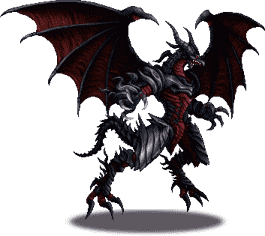
\includegraphics[width=0.3\columnwidth]{./art/jobs/bahamut.png}}
{
	HP: & \hfill 60 & MP: & \hfill 80\\
	STR: & \hfill 5 & DEF: & \hfill 4 \\
	MAG: & \hfill 4 & RES: & \hfill 4 \\
	AGI: & \hfill 3 & Size: & \hfill L\\
}
{
	\accf{Claw}: 3d DMG\\
	\accf{Immune}: All Status Effects \hfill \accf{Resilience:}\dark\fire
}
{
	\mreaction{Final Attack}{If you are about to fall to 0 HP you may use one of your abilities without cost or cast time before falling KO.}
	\mtech{Impulse \hfill \accf{Level 9}}{12}{0r}{3u}{Self}{All enemies in the target area suffer 3d dark damage.}{\dark}{}	
	\mtech{Obliterating Breath \hfill \accf{Level 9}}{14}{0r}{3u (front)}{3u}{Everyone in the target area makes a DC 8 check and suffers 3d damage as well as Poison and Blind for 3 rounds upon failure.}{\poison \blind}{}
	\mspell{Megaflare \hfill \accf{Level 10}}{25}{2r}{2u}{10u}{You deal 6d+40 damage to all enemies in the target area. The damage dealt ignores the target's RES.}{\fire}
}
%
\vfill
%
\ofmonster{Shiva}{5}{
\includegraphics[width=0.23\columnwidth]{./art/jobs/shiva.png}}
{
	HP: & \hfill 25 & MP: & \hfill 45\\
	STR: & \hfill 2 & DEF: & \hfill 1 \\
	MAG: & \hfill 3 & RES: & \hfill 4 \\
	AGI: & \hfill 2 & Size: & \hfill M\\
}
{
	\accf{Icicle}: 2d DMG, 2u Range  (increased to 3d at Level 8)\\
	\accf{Resilience}:\ice \hspace*{\fill} \accf{Weakness:}\fire
}
{	
	\mspell{Blizzard \hfill \accf{Level 5}}{4}{0r}{Single}{3u}{You deal 2d ice damage to the target.}{}
	\mspell{Deprotect \hfill \accf{Level 5}}{5}{0r}{Single}{5u}{The target suffers DeDEF for 3 rounds.}{\dedef}
	\mspell{Deshell \hfill \accf{Level 5}}{5}{0r}{Single}{5u}{The target suffers DeRES for 3 rounds.}{\deres}
	\mspell{Ice Wall \hfill \accf{Level 7}}{12}{0r}{3u (line)}{5u}{You create a 3u tall and wide wall of ice that blocks the path for 3 rounds. You cannot use this ability again as long as the previous wall still stands.}{}
	\mspell{Blizzaga \hfill \accf{Level 8}}{12}{1r}{Single}{5u}{You deal 6d ice damage to the target.}{\ice}
	\mspell{Diamond Dust \hfill \accf{Level 10}}{20}{0r}{3u (front)}{Self}{All enemies in the target area suffer 6d ice damage and Immobile for 1 round.}{\ice\immobile}		
}
\clearpage
%
%
%
%
%
\ofjob{Thief}
{
	\ofquote{"I PREFER the term ”treasure hunter!"\\}{Locke}\ofrow
	
\includegraphics[width=\columnwidth]{./art/jobs/thief.jpg}\ofrow
	\accf{Thieves} are mobile melee fighters, who excel at "borrowing" items from enemies and have a heightened sense for worthwhile business. 
}
{Dagger}{Light Armor}{
	Level 1: & HP +20 & MP~+19 & AGI~+4 \\
	Level 2: & HP~+5  & MP~+10  & STR~+1 & DEF~+1 \\
	Level 3: & \multicolumn{3}{l}{Archetype Attribute Bonus} \\
	Level 4: & HP~+10 & MP~+5  & STR~+1 & DEF~+1 \\
	Level 5: & HP~+10 & MP~+10 & STR~+1 &        \\ 
	Level 6: & HP~+5  & MP~+5  & DEF~+2 & RES~+1 \\ 
	Level 7: & HP~+10 & MP~+10 & STR~+1 &        \\ 
	Level 8: & HP~+10 & MP~+5  & RES~+2 &        \\ 
	Level 9: & HP~+5  & MP~+10 & STR~+2 &        \\ 
	Level 10:& HP~+10 & MP~+10  & DEF~+1 
}{
	\ofjobtech{Steal}{3}{0r}{Single}{1u}{Make a DC 7 check and "borrow" something from the target if you succeed. Roll 1d and the you get your Level times 20G on 1 or 2, a Potion on a 3, a Remedy on a 4, an Ether on a 5 and a Phoenix Down on a 6. The item may also be determined in any other way by the GM.}{}{1} \ofabilitygap
	\ofjobtech{Flee}{4}{0r}{3u}{Self}{You and all allies in the target area can move twice as fast when running away from enemies for 3 rounds.}{}{2} \ofabilitygap
	\ofjobtech{Poison Dart}{7}{0r}{Single}{4u}{The target makes a DC~8 check and suffers 1d damage and one of the following Status Effects of your choice for 3 rounds upon failure: Poison, Immobile, Sleep}{}{4}\ofabilitygap
	\ofjobtech{Vanish}{8}{0r}{Single}{Self}{You become invisible for up to  5 rounds or until you take an action. While invisible, you gain Blink and if you hit an Attack, you always score a Critical Hit.}{\blink}{6} \ofabilitygap
	\ofjobtech{Sticky Fingers}{6}{0r}{Single}{Self}{For the next 3 rounds, whenever you perform a successful Attack you can also use Steal on the same target without additional cost. Additionally, all items that you receive from Steal are doubled for this duration.}{}{8} \ofabilitygap
	\ofjobtech{Mirror Image}{23}{1r}{Single}{1u}{You create an exact copy of yourself that lasts for 3 rounds or until you create a new one. It acts with you on your turn, following your command. The clone can use the same abilities as you except this one.}{}{10}
}{
	\ofarchetypet{Ninja}
	{HP~+14 & MP~+11 & STR~+2}
	{\ofarchetypetecha{Throw}{4}{0r}{Single}{5u}{You throw a piece of equipment from your inventory on the target and deal an amount of damage depending on its equipment rank. The damage dealt is 1d for Beginner, 2d for Advanced and 3d for Expert level equipment. You can collect all thrown objects at the end of the battle.}{}}
	{\ofarchetypepassive{First Strike}{When an ally chooses you to take the next turn, you can immediately take it instead of waiting for a turn of the opposing party.}}
	{\ofarchetypereaction{Counter Attack}{When an enemy hits you with an Attack, you can immediately make an Attack on him if he is within range.}}
	{\ofarchetypetechb{Assassinate}{14}{0r}{Single}{3u}{Move to the target and make an Attack on him. If you hit, he makes a DC~7 check and suffers KO upon failure.}{\ko}}
}{
	\ofarchetypet{Treasure Hunter}
	{HP~+10 & MP~+20 & DEF~+1 & RES~+1}
	{\ofarchetypetecha{Quick Pockets}{6}{0r}{Single}{Self}{Make an Attack after which you can immediately use an Item.}{}}
	{\ofarchetypepassive{Gilionaire}{Whenever you deal damage to an enemy, you also receive an amount of Gil equal to the total damage dealt.}}
	{\ofarchetypereaction{Pickpocket}{Whenever you evade an Attack by an enemy, you can immediately use Steal on him without any cost.}}
	{\ofarchetypetechb{Gil Toss}{5}{0r}{Single}{5u}{Throw an amount of Gil on the target up to a maximum of 100G. The target suffers 1d damage for every 20G thrown. The money is destroyed in the process.}{}}
}
%
%
%
%
%
\ofjob{Tinker}
{
	\ofquote{"I don't give a rat's ass whether it's science or magical power. No, I guess if I had to choose, I'd rather put my money on the power of science."}{Cid}\\\\
	
\includegraphics[width=\columnwidth]{./art/jobs/tinker2.jpg}\ofrow
	\accf{Tinkers} are technical experts who defeat their enemies by using the power of science. 
	They can create special items and devices that cause fantastic effects in combat. 
	Tinkers prove that any sufficiently advanced technology is indistinguishable from magic.	
}
{Bow or Gun or Spear}{Robe}{
	Level 1: & HP~+17 & MP~+24 & AGI~+2 & STR~+1 \\
	Level 2: & HP~+5  & MP~+10 & RES~+1 & DEF~+1 \\
	Level 3: & \multicolumn{3}{l}{Archetype Attribute Bonus}  \\
	Level 4: & HP~+5  & MP~+10 & STR~+1 & DEF~+1 \\
	Level 5: & HP~+10 & MP~+10  & STR~+1 \\
	Level 6: & HP~+10 & MP~+10 & RES~+1 \\
	Level 7: & HP~+5  & MP~+10 & STR~+1 & DEF~+1 \\
	Level 8: & HP~+10 & MP~+10 & RES~+1 \\
	Level 9: & HP~+10 & MP~+10 & RES~+1 \\
	Level 10:& HP~+5  & MP~+10 & RES~+2
}{
	\ofjobtech{Stimulant}{4}{0r}{Single}{1u}{The target gains Regen for 3 rounds.}{\regen}{1}\ofabilitygap
	\ofjobtech{Flamethrower}{4}{0r}{3u (front)}{Self}{Make an Attack against every enemy in the target area. When you hit, the damage dealt is of fire type.}{\fire}{2}\ofabilitygap
	\ofjobtech{Propel}{6}{0r}{1u}{Self}{You shoot up to 3u into the air from where you can move and act as usual. After 2 rounds, you land on the ground in your current position.}{}{4}\ofabilitygap
	\ofjobtech{Fortify Position}{10}{0r}{2u}{5u}{You create a special field in the target area for 3 rounds. All allies gain EnSTR and EnDEF as long as they are standing inside it.}{\enstr\enndef}{6}\ofabilitygap	
	\ofjobtech{Shockwave}{9}{0r}{3u}{Self}{Everyone in the target area except you receives 3d damage and is pushed back by 3u. In addition, all affected targets make a DC~8 check and suffer Immobile for 1 round upon failure.}{\immobile}{8}\ofabilitygap
	\ofjobtech{Pandora's Box}{26}{1r}{5u}{Self}{All enemies in the target area suffer 4d damage. In addition, all affected targets roll 1d and suffer the following Status Effects for 3 rounds based on the result: 1-Immobile, 2-Slow, 3-Silence, 4-Poison, 5-Blind, 6-Sleep.}{\immobile\slow\silence\poison\blind\sleep}{10}
}{
	\ofarchetypet{Chemist}
	{HP~+8 & MP~+17 & RES~+2}
	{\ofarchetypetecha{Turbo Vaccine}{6}{0r}{Single}{1u}{The target regains 1d HP and becomes Immune to Poison, Silence, Blind and flu-like viruses for 3 rounds.}{}}
	{\ofarchetypepassive{Item Lore}{You can use Items in a range of up to 3u and you may affect everyone within 1u of the target. Both effects also apply to the Stimulant, Turbo Vaccine and Mix Techs.}}
	{\ofarchetypereaction{Auto-Potion}{Whenever you suffer damage, you can immediately use an Item. You can only use this effect once per round.}}
	{\ofarchetypetechb{Mix}{10}{0r}{Single}{3u}{Use 2 Items on the target and then roll 1d. Targeted allies recover 3d HP on 1-2, gain Blink for 3r on 3-4 and Haste for 3r on 5-6. Targeted enemies suffer 3d damage on 1-2, Immobile for 3r on 3-4 and Slow for 3r on 5-6.}{\blink\haste\immobile\slow}}
}{
	\ofarchetypet{Machinist}
	{HP~+10 & MP~+10 & STR~+2 & DEF~+1}
	{\ofarchetypetecha{Autoturret}{8}{0r}{1u}{1u}{You create a turret in the target area for 3 rounds. At the start of each turn, deal damage equal to your current Level to one enemy within 3u of it.}{}}
	{\ofarchetypepassive{Synthesis}{You gain an additional STR+1, DEF+1 or RES+1 for every Materia that you have equipped.}}
	{\ofarchetypereaction{Ballistic Defense}{Whenever you would suffer damage from an enemy that is further than 2u away from you, make a DC 7 check. If you succeed, the damage dealt is halved.}}
	{\ofarchetypetechb{Satellite Beam}{12}{0r}{?}{?}{All affected enemies suffer 5d damage. Choose one of the following target shapes to determine the affected targets: draw a 1u thick ring around you with an outer radius of up to 8u \accf{or} draw a 1u wide line with both ends within 8u of you \accf{or} all enemies within 5u of you make a check and everyone who rolls an odd number is affected.}{}}
}
%
%
%
%
%
\ofjob{Time Mage}
{
	\ofquote{"Time... It will not wait."\\}{Ultimecia}\\\\
	
\includegraphics[width=\columnwidth]{./art/jobs/timemage.jpg}\ofrow
	\accf{Time Mages} are masters of time and space, who understand that imagination is more important than knowledge. 
	They manipulate the flow of time and bend the fabric of reality to their advantage.
}
{Staff}{Robe}{
	Level 1: & HP~+17 & MP~+28 & AGI~+2 & MAG~+1 \\
	Level 2: & HP~+5  & MP~+10 & RES~+1 & STR~+1 \\
	Level 3: & \multicolumn{3}{l}{Archetype Attribute Bonus}  \\
	Level 4: & HP~+10  & MP~+10 & MAG~+1 &        \\ 
	Level 5: & HP~+10 & MP~+10 & RES~+1 &		  \\ 
	Level 6: & HP~+5  & MP~+10 & DEF~+1 & RES~+1 \\ 
	Level 7: & HP~+5  & MP~+10 & RES~+2 \\ 
	Level 8: & HP~+10  & MP~+10 & DEF~+1 \\ 
	Level 9: & HP~+5  & MP~+10 & RES~+2 &        \\ 
	Level 10:& HP~+5  & MP~+10 & MAG~+1 &	RES~+1	  
}{
	\ofjobspell{Gravity}{6}{0r}{Single}{3u}{The target suffers 2d damage and can only move half his usual distance on his next turn.}{}{1}\ofabilitygap
	\ofjobspell{Haste}{8}{0r}{Single}{5u}{The target gains Haste for 3 rounds.}{\haste}{2}\ofabilitygap
	\ofjobspell{Slow}{8}{0r}{Single}{5u}{The target suffers Slow for 3 rounds.}{\slow}{2}\ofabilitygap
	\ofjobspell{Float}{8}{0r}{Single}{3u}{The target levitates up to 3u above the ground for 2 rounds. While allies can still move in the air, targeted enemies suffer Immobile for the duration.}{}{4}\ofabilitygap
	\ofjobspell{Graviga}{15}{1r}{2u}{6u}{All enemies in the target area suffer 6d damage and a Slow Field appears in the target area that lasts for 3 rounds.}{}{6}\ofabilitygap
	\ofjobspell{Stop}{16}{0r}{30u}{Self}{All enemies in the target area make a DC 8 check and suffer Sleep for 1 round upon failure.}{\sleep}{8}\ofabilitygap
	\ofjobspell{Banish}{26}{0r}{Single}{5u}{Temporarily banish the target into another dimension. If he is an ally, he can still take turns, but not interact with the battlefield. After 3 rounds, the target reappears in the same spot, anyone in the same space is pushed aside and suffers 6d damage. You cannot use Banish consecutively on the same target or if a previous cast is still active.}{}{10}
}{
	\ofarchetypet{Illusionist}
	{HP~+5 & MP~+20 & MAG~+2}
	{\ofarchetypespella{Warp}{6}{0r}{1u}{5u}{You teleport to an unoccupied location of your choice that you can see within 5u.}{}}
	{\ofarchetypepassive{Tunneling}{Whenever you cast a spell, you can choose to double its range and target distance by also doubling its MP cost.}}
	{\ofarchetypereaction{Quick Warp}{Whenever you are targeted by an Attack, you can attempt to Warp. In this case, you make the evasion check with advantage and if you succeed, the Warp spell takes effect in addition to the evasion. In either case, you have to respect the spell's MP cost.}}
	{\ofarchetypespellb{Exchange}{14}{0r}{Single}{10u}{Choose two targets within range and exchange their positions. Targeted enemies suffer an additional 4d damage. Targeted allies instead cause 4d damage to everyone within 2u of their new position. Also, both targets push aside anything that would obstruct their new spot.}{}}
}{
	\ofarchetypet{Oracle}
	{HP~+8 & MP~+17 & STR~+1 & RES~+1}
	{\ofarchetypespella{Extend}{5}{0r}{Single}{5u}{The duration of all Status Effects that the target is suffering or benefiting from, is extended by 3 rounds.}{}}
	{\ofarchetypepassive{Read Ahead}{Right before the start of each combat, you can take one extra turn, even if the enemy has a surprise round.}}
	{\ofarchetypereaction{Kismet}{Whenever a spell or tech that targets someone within 5u takes effect, you can choose to delay it. In this case, the battle continues as usual and the ability instead takes effect on the target after 1 round.}}
	{\ofarchetypespellb{Quicken}{10}{0r}{Single}{5u}{The target takes an extra turn immediately before yours is finished. The round continues as usual afterwards, so you still have to pick the next combatant for your side. You can only use this ability once per round.}{}}
}
%
%
%
%
%
\ofjob{Warrior}
{
	\ofquote{"I dreamt I was a moron."\\}{Squall}\\\\
	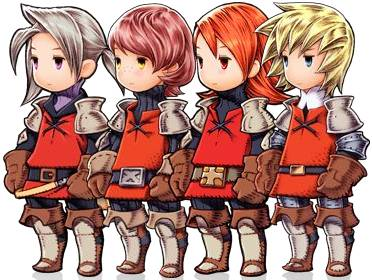
\includegraphics[width=\columnwidth]{./art/jobs/warrior.jpg}\ofrow
	\accf{Warriors} are specialists in melee combat, because of their strong physical offense and defense. 
	They are proficient with powerful swords and armor, allowing them to become even more dangerous and durable. 
}
{Sword}{Light or Heavy Armor}{
	Level 1: & HP +25 & MP~+18 & AGI~+3 & STR +1 \\
	Level 2: & HP~+10 & MP~+5  & STR~+1 & DEF~+1 \\
	Level 3: & \multicolumn{3}{l}{Archetype Attribute Bonus}  \\
	Level 4: & HP~+10 & MP~+5  & STR~+2 &        \\ 
	Level 5: & HP~+10  & MP~+10 & DEF~+1 \\ 
	Level 6: & HP~+10 & MP~+5  & DEF~+1 & RES~+1 \\ 
	Level 7: & HP~+10 & MP~+10  & STR~+1 &        \\ 
	Level 8: & HP~+10 & MP~+5  & RES~+2 &        \\ 
	Level 9: & HP~+5  & MP~+10 & STR~+1 & DEF~+1 \\ 
	Level 10:& HP~+10 & MP~+5  & DEF~+2 &         
}{
	\ofjobtech{Rush}{3}{0r}{Single}{1u}{Make an Attack against the target. If you hit, you push him back by 1u on top of the damage dealt.}{}{1}\ofabilitygap
	\ofjobtech{Beatdown}{6}{0r}{Single}{1u}{Make an Attack where the target has Advantage on the evasion check. If you hit, you score a Critical Hit.}{}{2}\ofabilitygap
	\ofjobtech{Vitality}{4}{0r}{Single}{Self}{For the next 3 rounds, when an effect restores your HP or MP, the amount is doubled. Also, when you have to make a check to resist a negative effect, its DC is reduced by 2.}{}{4}\ofabilitygap
	\ofjobtech{Army of One}{10}{0r}{3u}{Self}{Make an Attack against every enemy in the target area by making one damage roll that applies to all affected targets that fail to evade. After using the ability, you can move next to any of the affected targets.}{}{6}\ofabilitygap
	\ofjobtech{Bravery}{10}{0r}{2u}{Self}{You and all allies within the target area gain EnSTR and EnMAG for 2 rounds.}{\enstr \enmag}{8}\ofabilitygap
	\ofjobtech{Omnislash}{28}{0r}{Single}{1u}{Make 3 separate Attacks against the target. Each time he rolls 4 or less on an evasion check, you score a Critical Hit.}{}{10}
}{
	\ofarchetypet{Dark Knight}
	{HP~+5 & MP~+15 & DEF~+1 & RES~+2}
	{\ofarchetypetecha{Defensebreak}{6}{0r}{Single}{1u}{Make an Attack on the target. If you hit, he suffers DeDEF and DeRES for 2 rounds on top of the damage dealt.}{\dedef \deres}}
	{\ofarchetypepassive{Souleater}{Whenever you successfully Attack an enemy, you can additionally inflict dark damage equal to half of the total damage dealt, to yourself and all enemies within~3u.}}
	{\ofarchetypereaction{Blood Price}{Whenever an enemy that you can see spends MP, you can force him to spend an equal amount of HP instead if he has enough HP to do so. Afterwards, increase your own HP by half the amount spent.}}
	{\ofarchetypetechb{Berserk}{10}{0r}{Single}{5u}{For the next 3 rounds the target can only take the Attack action, but every successful Attack is a Critical Hit. If you target an enemy with this ability, he makes a DC~8 check and only suffers this effect upon failure.}{}}
}{
	\ofarchetypet{Samurai}
	{HP~+16 & MP~+9 & STR~+2}
	{\ofarchetypetecha{Focus}{5}{0r}{Target}{Self}{For the next 3 rounds, whenever you Attack an enemy, he has Disadvantage on the the evasion check.}{}}
	{\ofarchetypepassive{Cripple}{Whenever the target of your Attacks rolls a 5 or less on the evasion check he additionally suffers one of the following Status Effects of your choice for 1 round upon failure: Immobile, Blind, DeSTR.}}
	{\ofarchetypereaction{Bushido}{You can evade Techs by passing an evasion check the same way that you evade Attacks. Also, whenever you evade an Attack or Tech, you regain an amount of MP equal to your current Level.}}
	{\ofarchetypetechb{Razor Gale}{8}{0r}{5u (line)}{Self}{Everyone in the target area suffers 4d wind damage.}{\wind}}
}
%
%
%
%
%
\ofjob{White Mage}
{
	\ofquote{"Hey, that’s Cloud’s line! ’It’s too dangerous, I can’t get you involved...' Blah blah blah."\\}{Aerith}\\\\
	
\includegraphics[width=\columnwidth]{./art/jobs/whitemage.jpg}\ofrow
	\accf{White Mages} are experts of defensive magic and boast a variety of recovery and protective spells.
	While mediocre in physical combat, they also feature incredible resistance against magic. 
}
{Staff}{Robe}{
	Level 1: & HP~+19 & MP~+25 & AGI~+2 & STR~+1 \\
	Level 2: & HP~+5  & MP~+10 & MAG~+1 & RES~+1 \\
	Level 3: & \multicolumn{3}{l}{Archetype Attribute Bonus} \\
	Level 4: & HP~+10 & MP~+5 & MAG~+1 & DEF~+1	  \\
	Level 5: & HP~+5  & MP~+10 & RES~+1 &	STR~+1  \\ 
	Level 6: & HP~+5  & MP~+5 & MAG~+2 &        \\ 
	Level 7: & HP~+10  & MP~+10 & RES~+1 & DEF~+1 \\ 
	Level 8: & HP~+5 & MP~+5  & MAG~+2 & DEF~+1 \\ 
	Level 9: & HP~+5  & MP~+10 & RES~+1 &	MAG~+1   \\ 
	Level 10:& HP~+10 & MP~+10 & RES~+1 &	        
}{	
	\ofjobspell{Cure}{4}{0r}{Single}{3u}{The target regains 2d HP.}{}{1}\ofabilitygap
	\ofjobspell{Drain}{6}{0r}{Single}{3u}{Deal 1d damage to the target and increase your own HP by the total amount of damage dealt.}{}{2}\ofabilitygap
	\ofjobspell{Esuna}{6}{0r}{Single}{5u}{You remove all negative Status Effects except KO from the target.}{}{4}\ofabilitygap
	\ofjobspell{Curaga}{14}{1r}{2u}{5u}{Everyone in the target area regains 6d HP.}{}{6}\ofabilitygap
	\ofjobspell{Clear}{6}{0r}{5u}{50u}{You remove one active Field Effect within range.}{}{6}\ofabilitygap
	\ofjobspell{Holy}{21}{2r}{Single}{12u}{You deal 6d+45 holy damage to the target.}{\holy}{8}\ofabilitygap
	\ofjobspell{Auto-Life}{28}{2r}{Single}{3u}{You summon a guardian angel that watches over the target. The next time he falls KO, he is instantly revived with 1 HP. This effect does not stack and if not activated, it expires when the target goes to sleep.}{\ko}{10}
}{
	\ofarchetypet{Sage}
	{HP~+11 & MP~+9 & MAG~+2 & STR~+1}
	{\ofarchetypespella{Sleep}{6}{0r}{Single}{5u}{The target makes a DC 8 check and suffers Sleep for 3 rounds upon failure.}{\sleep}
		\vspace*{0.1cm}\\ \ofarchetypespella{Silence}{6}{0r}{Single}{5u}{The target makes a DC 8 check and suffers Silence for 3 rounds upon failure.}{\silence}}
	{\ofarchetypepassive{Ancient Wisdom}{Whenever you inflict on or more Status Effects on a target, you can also inflict DeDEF or DeRES on him for 3 rounds.}}
	{\ofarchetypereaction{Absorb MP}{When you are the target of an enemy ability, increase your MP by half the amount that the caster spent on it.}}
	{\ofarchetypespellb{Curse}{14}{1r}{Single}{5u}{The target makes a DC~9 check and upon failure he suffers 4d damage as well as Poison and Zombie for 3 rounds.}{}}
}{
	\ofarchetypet{Medic}
	{HP~+7 & MP~+13 & RES~+2 & DEF~+1}
	{\ofarchetypespella{Protect}{4}{0r}{Single}{5u}{The target gains EnDEF for 3 rounds.}{\enndef} \vspace*{0.1cm}\\ \ofarchetypespella{Shell}{4}{0r}{Single}{5u}{The target gains EnRES for 3 rounds.}{\enres}}
	{\ofarchetypepassive{Doctor's Code}{Whenever you use Magic on an ally within 1u, you can also immediately use an Item on him in addition.}}
	{\ofarchetypereaction{No Collateral}{Whenever you would be affected by a spell or tech that you are not the primary target of, you can choose that you and all other secondary targets are unaffected.}}
	{\ofarchetypespellb{Full-Life}{22}{2r}{Single}{5u}{You remove the KO status from the target and fully restore his HP.}{\ko}}
}